% LOrkCraft Paper for NIME 2013 
%
% Using the LaTeX Template for NIME 2013

\documentclass{nime-document-class}

\begin{document}

\conferenceinfo{NIME'13,}{May 27 -- 30, 2013, KAIST, Daejeon, Korea.}

% use \projectName{} to refer to the project in the paper
% makes changing it later much easier - just change it here!
\newcommand{\projectName}{LOrkCraft}

\title{\projectName{}: Making Music While Playing Starcraft 2}

\numberofauthors{3}
\author{
% 1st. author
\alignauthor
Mark Cerqueira\\
       \affaddr{Smule, Inc.}\\
       \affaddr{577 College Avenue}\\
       \affaddr{Palo Alto, California}\\
       \email{mark@smule.com}
% 2nd. author
\alignauthor
Spencer Salazar\\
       \affaddr{Center for Computer Research in Music and Acoustics (CCRMA)}\\
       \affaddr{Stanford University}\\
       \email{spencer@ccrma.stanford.edu}
% 3rd. author
\alignauthor
Ge Wang\\
       \affaddr{Center for Computer Research in Music and Acoustics (CCRMA)}\\
       \affaddr{Stanford University}\\
       \email{ge.stanford.edu}
}

\maketitle
\begin{abstract}
\projectName{} is a collection of utilities that enable real-time data gathering from a Starcraft 2 match to external audio servers via Open Sound Control allowing the match itself to become a live performance piece.
This paper details the technical and aesthetic decisions made during the development of \projectName{}, covering data collected during the game and discussing the sonic mappings explored.
\end{abstract}

\keywords{NIME, Starcraft 2, sonification, music}

\section{Introduction}
Introduce Starcraft 2 and the premise for taking game data and making music with it.

\section{Background}
Talk about background.

\section{Related Work}
Discuss previous work.

\section{System Overview}
\projectName{} consists of a set of utilities that work in tandem to get data from a live Starcraft 2 match to OSC clients that sonify the game.
The main components include a custom Starcraft 2 map, a Ruby parser and OSC dispatcher, and our audio engine.

\subsection{Creating the Custom Map}
An existing Starcraft 2 map, Antiga Shipyard created by Blizzard shown in (Figure~\ref{fig:AntigaShipyardFigure}), was modified to collect various data in real-time during a game.
These {\em triggers} fire off either periodically (every 2 seconds) or after certain events (a unit is produced). When a trigger fires, data is collected and written to XML bank files.
The map created for \projectName{} is for two players, but the triggers can be shared to any other map with any number of players. 

\begin{figure}[htbp]
	\centering
		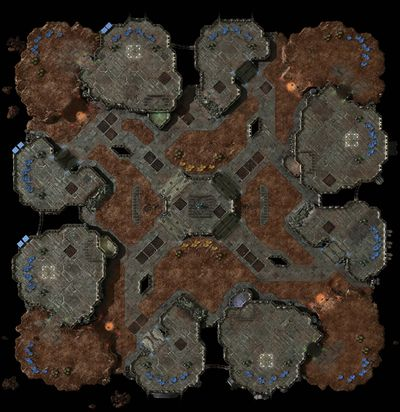
\includegraphics[width=1\columnwidth]{antiga-shipyard}
	\caption{The Antiga Shipyard map. Players start in the bottom right or top left positions.}
	\label{fig:AntigaShipyardFigure}
\end{figure}


Data collected during the game focuses on player actions and current state of the player's army.
Tracked data includes:
\begin{itemize} \itemsep1pt \parskip0pt \parsep0pt
  \item Coordinates where a player is currently focused on the map
  \item Composition of the player's standing army
  \item Units being produced by the player and their current build progress
  \item The player's effective actions per minute (APM)
  \item Various metrics about a player's economic health including mineral and vespene gas collection rate as well as harvesters built and lost
  \item Total number of enemy units destroyed and structures razed
  \item The player's general {/em score} that combines all these factors to produce a single number that is normally a good indicator of performance (this is typically only shown after a match has ended) \ldots
\end{itemize}

\subsection{Parsing and Sending Game Data}
A Ruby script monitors the directories that contain these bank files using guard/listen and when the files are updated, the data is parsed out of the XML bank files using Nokogiri and that data is sent to any listening OSC clients that handle sonification or visualization.
Unfortunately, this is the only {\em legitimate} way to get data out of Starcraft 2, but we found the latency between a trigger being fired and an OSC client receiving the message to be acceptable given we had fine control over how often our script polls the file system for bank file updates.
With OS-specific file system polling adapters, the overhead of writing to a file and parsing the data out of that file became negligible in tests.

\subsection{Sonification of Game Data}
What we did with the OSC messages.

\subsection{Conclusion}
What we want people to do with \projectName{}.

% Acknowledgments are optional
\section{Acknowledgments}
We would like to thank Tasteless and Artosis for being awesome.

% Place this command where you want to balance the columns on the last page. 
% \balancecolumns 

\end{document}
